\de{ĐỀ THI HỌC KỲ II NĂM HỌC 2022-2023}{THPT Trường Chinh}


\begin{bt}%[0D7B3-2]%[Dự án đề kiểm tra HKII NH22-23- Vuc Ngọc Hảo]%[THPT Trường Chinh]
Giải bất phương trình: $2 \sqrt{2 x^2-3 x-1}=x+2$. 
	\loigiai{
	\[	\begin{aligned}
	&	2 \sqrt{2 x^2-3 x-1}=x+2\\
		\Leftrightarrow & \heva{&x+2\geq 0\\&4(2x^2-3x-1)=(x+2)^2}\\
			\Leftrightarrow & \heva{&x\geq-2 \\&7x^2-16x-8=0}\\
			\Leftrightarrow & \heva{&x\geq-2 \\&7x^2-16x-8=0}\\
				\Leftrightarrow & \hoac{&x=\dfrac{8+2\sqrt{30}}{7}\\&x=\dfrac{8-2\sqrt{30}}{7}.}
		\end{aligned}\]
		
}
\end{bt}


\begin{bt}%[0D8B2-2]%[Dự án đề kiểm tra HKII NH22-23- Vuc Ngọc Hảo]%[THPT Trường Chinh]
Từ các chữ số $0;1;2;3;4;5;6;7$ có thể lập được bao nhiêu số tự nhiên lẻ có $4$ chữ số khác nhau?
	\loigiai{Gọi $\overline{abcd}$ là số cần lập.\\
		Chọn $d$ có $4$ cách.\\
		Chọn $a\ne 0$ và $a\ne d$ có $6$ cách.\\
		Chọn $b,c$ có $\mathrm{A}_6^2$ cách.\\
		Vậy có $4\cdot 6\cdot \mathrm{A}_6^2=720$ số.}
\end{bt}


\begin{bt}%[0D8YO-1]%[Dự án đề kiểm tra HKII NH22-23- Vuc Ngọc Hảo]%[THPT Trường Chinh]
	Khai triển Nhị thức $(1-x)^4$, sau đó tìm hệ số của $x^4$.
	\loigiai{$(1-x)^4=\mathrm{C}_4^0(-x)^0+\mathrm{C}_4^1(-x)^1+\mathrm{C}_4^2(-x)^2+\mathrm{C}_4^3(-x)^3+\mathrm{C}_4^4(-x)^4=1-4x+6x^2-4x^3+x^4$.\\
	Hệ số của $x^4$ là $1$.
}
\end{bt}


\begin{bt}%[0D9KQ-5]%[Dự án đề kiểm tra HKII NH22-23- Vuc Ngọc Hảo]%[THPT Trường Chinh]
	Một hộp đựng $6$ viên bi xanh và $4$ viên bi đỏ (các bi đều khác nhau).
	\begin{enumerate}
		\item Lấy ngẫu nhiên $3$ bi, tính xác suất để trong $3$ bi được chọn có đủ $2$ màu?
		\item Lấy cả $10$ bi trên sắp xếp ngẫu hiên thành 1 hàng. Tính xác suất của biến cố \lq\lq cùng màu thì kề nhau\rq\rq.
	\end{enumerate}
	\loigiai{\begin{enumerate}
		\item $n(\Omega)=\mathrm{C}_{10}^3=120$.\\
		Gọi $A$ là biến cố \lq\lq lấy được $3$ viên bi đủ $2$ màu\rq\rq.\\
		TH1: Lấy được $2$ viên bi xanh và $1$ viên bi đỏ có $\mathrm{C}_6^2\cdot \mathrm{C}_4^1$ cách.\\
		TH2: Lấy được $1$ viên bi xanh và $2$ viên bi đỏ có $\mathrm{C}_6^1\cdot \mathrm{C}_4^2$ cách.\\
		Suy ra $n(A)=\mathrm{C}_6^2\cdot \mathrm{C}_4^1+\mathrm{C}_6^1\cdot \mathrm{C}_4^2=96$.
		Vậy $\mathrm{P}(A)=\dfrac{n(A)}{n(\Omega)}=\dfrac{96}{120}=\dfrac{4}{5}$.
		\item  $n(\Omega)=10!$.\\
		Gọi $B$ là biến cố \lq\lq cùng màu thì kề nhau\rq\rq.\\
		Vì bi cùng màu phải kề nhau nên coi $6$ viên bi xanh là bi xanh, $4$ viên bi đỏ là bi đỏ.\\
		Số cách xếp $2$ loại bi xanh đỏ là $2!$.\\
		Số cách xếp $6$ viên bi xanh là $6!$.\\
		Số cách xếp $4$ viên bi đỏ là $4!$.\\
		Suy ra có $2!\cdot 6!\cdot4!$ cách xếp.\\
		Vậy $\mathrm{P}(B)=\dfrac{n(B)}{n(\Omega)}=\dfrac{2!\cdot 6!\cdot4!}{10!}=\dfrac{1}{105}$.
		\end{enumerate}
		
	}
\end{bt}


\begin{bt}%[0H7KI-2]%[Dự án đề kiểm tra HKII NH22-23- Vuc Ngọc Hảo]%[THPT Trường Chinh]
	Trên hệ trục tọa độ $Oxy$ cho $\triangle ABC$ biết $A(-1;4)$, $B(3;2)$, $C(2;1)$.
	\begin{enumerate}
		\item Viết phương trình tổng quát của đường thẳng $AB$.
		\item Xác định tọa độ trực tâm của $\triangle ABC$.
	\end{enumerate}
	\loigiai{
	\begin{enumerate}
\item Đường thẳng $AB$ có véc-tơ chỉ phương $\overrightarrow{u}=\overrightarrow{AB}=(4,-2)$ suy ra véc-tơ pháp tuyến của đường thẳng $AB$ là $\overrightarrow{n}=(1;2)$.\\
Phương trình tổng quát của đường thẳng $AB$ là $$1(x+1)+2(y-4)=0\Leftrightarrow x+2y-7=0.$$
\item Kẻ $AM\perp BC, (M\in BC)$, $BN\perp AC, (N\in AC)$.\\
Khi đó ta có trực tâm $H=AM\cap BN$.\\
Đường thẳng $AM$ đi qua điểm $A(-1;4)$ và có véc-tơ pháp tuyến $\overrightarrow{n}=\overrightarrow{CB}=(1;1)$ có phương trình là $$1\cdot (x+1)+1\cdot (y-4)=0\Leftrightarrow x+y-3=0.$$
	Đường thẳng $BN$ đi qua điểm $B(3;2)$ và có véc-tơ pháp tuyến $\overrightarrow{n}=\dfrac{1}{3}\overrightarrow{AC}=(1;-1)$ có phương trình là $$1\cdot (x-3)-1\cdot (y-2)=0\Leftrightarrow x-y-1=0.$$
	Tọa độ điểm $H$ là nghiệm của hệ phương trình
	$$\heva{&x+y-3=0\\&x-y-1=0}\Leftrightarrow\heva{&x=2\\&y=1.}$$
	Vậy $H(2;1)$.
\end{enumerate}}
\end{bt}


\begin{bt}%[0H7BK-2]%[0H7BK-3]%[Dự án đề kiểm tra HKII NH22-23- Vuc Ngọc Hảo]%[THPT Trường Chinh]
	Trên hệ trục tọa độ $Oxy$ cho $M(-2;1)$, $N(4;3)$.
	\begin{enumerate}
		\item Viết phương trình đường tròn $(C)$ có tâm $M$ và qua $N$.
		\item Viết phương trình tiếp tuyến với đường tròn $(C)$ tại $N$.
	\end{enumerate}
	\loigiai{\begin{enumerate}
			\item Đường tròn $(C)$ có bán kính $R = MN = \sqrt{(4+2)^2 + (3-1)^2} = 2\sqrt{10}$.\\
			Phương trình đường tròn $(C)$ có tâm $M$ và qua $N$ có dạng:
			$(x+2)^2 +(y-1)^2 = 40$.
			\item Ta có $\vec{MN} = (6;2) \Rightarrow \vec{n}=(3;1)$.\\
			Phương trình tiếp tuyến tại $N(4;3)$ nhận $\vec{n}=(3;1)$ làm véc-tơ pháp tuyến có dạng:
			$$
			\begin{aligned}
			& 3(x-4) + 1(y-3) = 0 \\
			\Leftrightarrow \quad& 3x+y-15 = 0.
			\end{aligned}
			$$ 
		\end{enumerate}	
	}
\end{bt}
\begin{bt}%[0H7BL-2]%[Dự án đề kiểm tra HKII NH22-23- Vuc Ngọc Hảo]%[THPT Trường Chinh]
	Viết phương trình của elip $(E)$ biết $(E)$ có độ dài trục lớn là $10$ và độ dài trục nhỏ là $8$.
	\loigiai{Ta có độ dài trục lớn $2a = 10 \Leftrightarrow a=5$.\\  Độ dài trục nhỏ $2b=8 \Leftrightarrow b=4$.\\
		Suy ra phương trình elip $(E)$ có dạng: $\dfrac{x^2}{25} +\dfrac{y^2}{16} =1$.}
\end{bt}


\begin{bt}%[0D7K3-2]%[Dự án đề kiểm tra HKII NH22-23- Vuc Ngọc Hảo]%[THPT Trường Chinh]
Một mảnh vườn trồng hoa có hình dạng là một tam giác vuông. Biết tam giác vuông này có độ dài của hai cạnh góc vuông hơn kém nhau là $1$ m và chu vi của tam giác vuông này bằng $12$ m. Hãy tính diện tích của mảnh vườn trồng hoa đó. 
	\loigiai{Giả sử độ dài một cạnh góc vuông (cạnh nhỏ) của mảnh vườn có độ dài là $x, (x<12)$.\\
		Độ dài cạnh góc vuông còn lại là $x+1$.\\
		Suy ra cạnh huyền của mảnh vườn có độ dài là 
		$\sqrt{x^2 + (x+1)^2}$. (Áp dụng định lý Pi-ta-go)\\
		Chu vi của mảnh vườn bằng $12$ nên ta có:	
		$$
		\begin{aligned}
		& x + x + 1 + \sqrt{x^2 + (x+1)^2} = 12\\
		\Leftrightarrow \quad & \sqrt{2x^2 +2x +1} =11- 2x \\
		\Leftrightarrow \quad & 2x^2 +2x +1 = 121- 44x +4x^2 \quad \left(x \leq \dfrac{11}{2}\right)\\
		\Leftrightarrow \quad & 2x^2 -46x +120 =0\\
		\Leftrightarrow \quad & \hoac{& x=3 \,(\text{nhận})\\& x=20 \,(\text{loại}).}
		\end{aligned}
		$$ 
		Độ dài hai cạnh góc vuông của mảnh vườn lần lượt là $3$ và $4$.\\
		Suy ra diện tích của mảnh vườn trồng hoa $S = \dfrac{1}{2}\cdot3\cdot 4 =6$.}
\end{bt}


\begin{bt}%[0H9B4-0]%[Dự án đề kiểm tra HKII NH22-23- Vuc Ngọc Hảo]%[THPT Trường Chinh]
	Một khung tranh hình chữ nhật $MNPQ$, bên trong có gắn 1 bức tranh hình elip được đặt trong hệ trục tọa độ $Oxy$ như hình vẽ. Biết $O$ của elip trùng với tâm hình chữ nhật, $MN\parallel PQ \parallel B_2 B_1$, $MN$ đi qua $A_1$, $PQ$ đi qua $A_1$, $MQ\parallel NP \parallel A_1 A_2$, $MQ$ đi qua $B_1$, $NP$ đi qua $B_1$ với $A_1$, $A_2$, $B_1$, $B_2$ là các đỉnh của elip. Phương trình của elip là $\dfrac{x^2}{25}+\dfrac{y^2}{16}=1$. Tính chu vi hình chữ nhật $MNPQ$.
	\begin{center}
		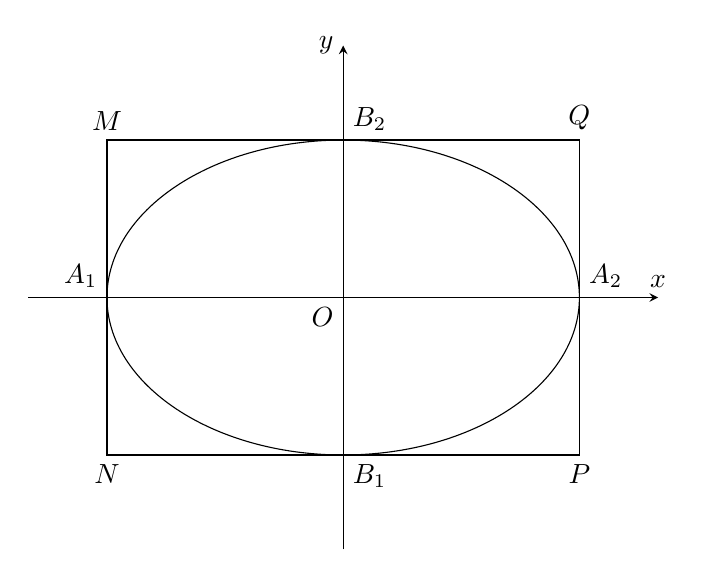
\begin{tikzpicture}
			\pgfmathsetmacro\a {sqrt(5)}
			\pgfmathsetmacro\b {sqrt(3)}  		
			\draw (0,0) ellipse ({3} and {2});
			\path 	(0,0) coordinate (O);
			\node[below left] at (0,0) {$O$};
			\node[above left] at (-3,0) {$A_1$};\node[above right] at (3,0) {$A_2$};\node[below right] at (0,-2) {$B_1$};\node[above right] at (0,2) {$B_2$};
		
			\draw[-stealth] (-4,0)--(4,0)node[above]{$x$};
			\draw[-stealth] (0,-3.2)--(0,3.2)node[left]{$y$};
			\draw (-3,2) node[above]{$M$}--(3,2)node[above]{$Q$}--(3,-2)node[below]{$P$}--(-3,-2)node[below]{$N$}--cycle;

		\end{tikzpicture}
	\end{center}
	\loigiai{Từ phương trình elip $\dfrac{x^2}{25}+\dfrac{y^2}{16}=1$, ta suy ra $a=5, b=4$.\\
		Khi đó độ dài trục lớn, trục bé lần lượt là: $2a= 2{,}5 = 10$; $2b = 2{,}4 = 8$. \\
		Chu vi hình chữ nhật $MNPQ$ là $C= 2(MN+MQ) = 2(8 + 10) = 36$.}
\end{bt}



